\documentclass[11pt]{article}
\usepackage[margin=1.1in]{geometry}
\usepackage{mathptmx}
\usepackage{amsmath,amssymb}
\usepackage{graphicx}
\usepackage{booktabs}
\usepackage{caption}
\usepackage[colorlinks=true,linkcolor=black,citecolor=black,urlcolor=blue]{hyperref}
\usepackage{titlesec}
\usepackage{xcolor}

\captionsetup{font=small,labelfont=bf}
\titleformat{\section}{\large\bfseries}{\thesection}{0.7em}{}
\titleformat{\subsection}{\normalsize\bfseries}{\thesubsection}{0.7em}{}

\newcommand{\keyfinding}[1]{\vspace{2pt}\noindent\fbox{\parbox{0.97\linewidth}{#1}}\vspace{2pt}}

\title{\bf A Memory That Only Looks Like One:\\[2pt]
\large The Recurrent State of a Hybrid Vision-Language Model Relays\\
the Picture Rather Than Storing It}

\author{Vizuara Research}
\date{August 2026}

\begin{document}
\maketitle

\begin{abstract}
\noindent
In a transformer an image persists: it becomes hundreds of key-value entries
that any later computation can attend to. In a hybrid linear-attention model it
does not. Most layers compress what they read into a fixed-size recurrent state
that later tokens overwrite. It is already known that recurrent models are
worse than transformers at retrieving from context, and that a fixed-size state
is the reason. What is not known is \emph{when} a particular model forgets,
\emph{what} it keeps while forgetting, and \emph{what breaks} downstream as a
consequence. We answer all three for Zamba2-VL-7B, whose 81 decoder layers all
carry a Mamba2 mixer while only 13 additionally carry attention.

First, at the moment of writing the recurrent state is highly informative about
\emph{which} object is present and close to uninformative about \emph{how many}
or \emph{where}: it records gist, not particulars. A probe on the best single
layer reads object identity at $92.5\%$ against a $12.5\%$ chance rate.

Second, the horizon over which that state genuinely retains its own past can be
computed before any experiment. Mamba2 multiplies the state by
$\exp(\Delta_t A)$ at every step, so retention after $k$ tokens is
$\exp(A\sum\Delta_t)$ and the per-head half-life is
$\ln 2/(|A|\bar{\Delta})$. Across three model scales the median predicted
half-life is $6.6$, $2.9$ and $2.6$ tokens, with nothing fitted.

Third, and this is the paper's central result, what a probe reads from that
state at distance is largely not retention. Splitting heads into thirds by
predicted half-life inverts the expected ordering: heads with a two-token
half-life decode identity at $61.7\%$ after sixty-four tokens, which retention
cannot produce. Evicting the visual key-value entries immediately after the
image, before any subsequent token is processed and without touching the
recurrent state, drops those heads from $51.6\%$ to $7.8\%$ at thirty-two
tokens, below chance, while leaving slow heads at distance zero nearly
unaffected. How much a head's readout depends on the attention channel is
itself predicted by that head's decay rate, correlating at $r = 0.991$ across
the three strata. The recurrent channel relays what attention is holding rather
than storing it, and the weights say which heads relay most.

This resolves the causal result. Exchanging all 81 recurrent states between two
runs that saw different images leaves $100$ of $100$ answers following the
host's own image, with every swap verified, whereas exchanging seven of the
thirteen attention caches moves $94$ of $100$ to the donor's image. The
recurrent swap cannot matter because it is overwritten within a few tokens from
the channel it does not touch. Finally, the redundancy premise behind visual
token and key-value pruning survives on this architecture down to a quarter of
the entries, but the cost of pruning harder roughly doubles with distance:
removing every visual entry costs $34$ accuracy points beside the image and
$59$ at thirty-two tokens.
\end{abstract}

\begin{figure}[t]
\centering
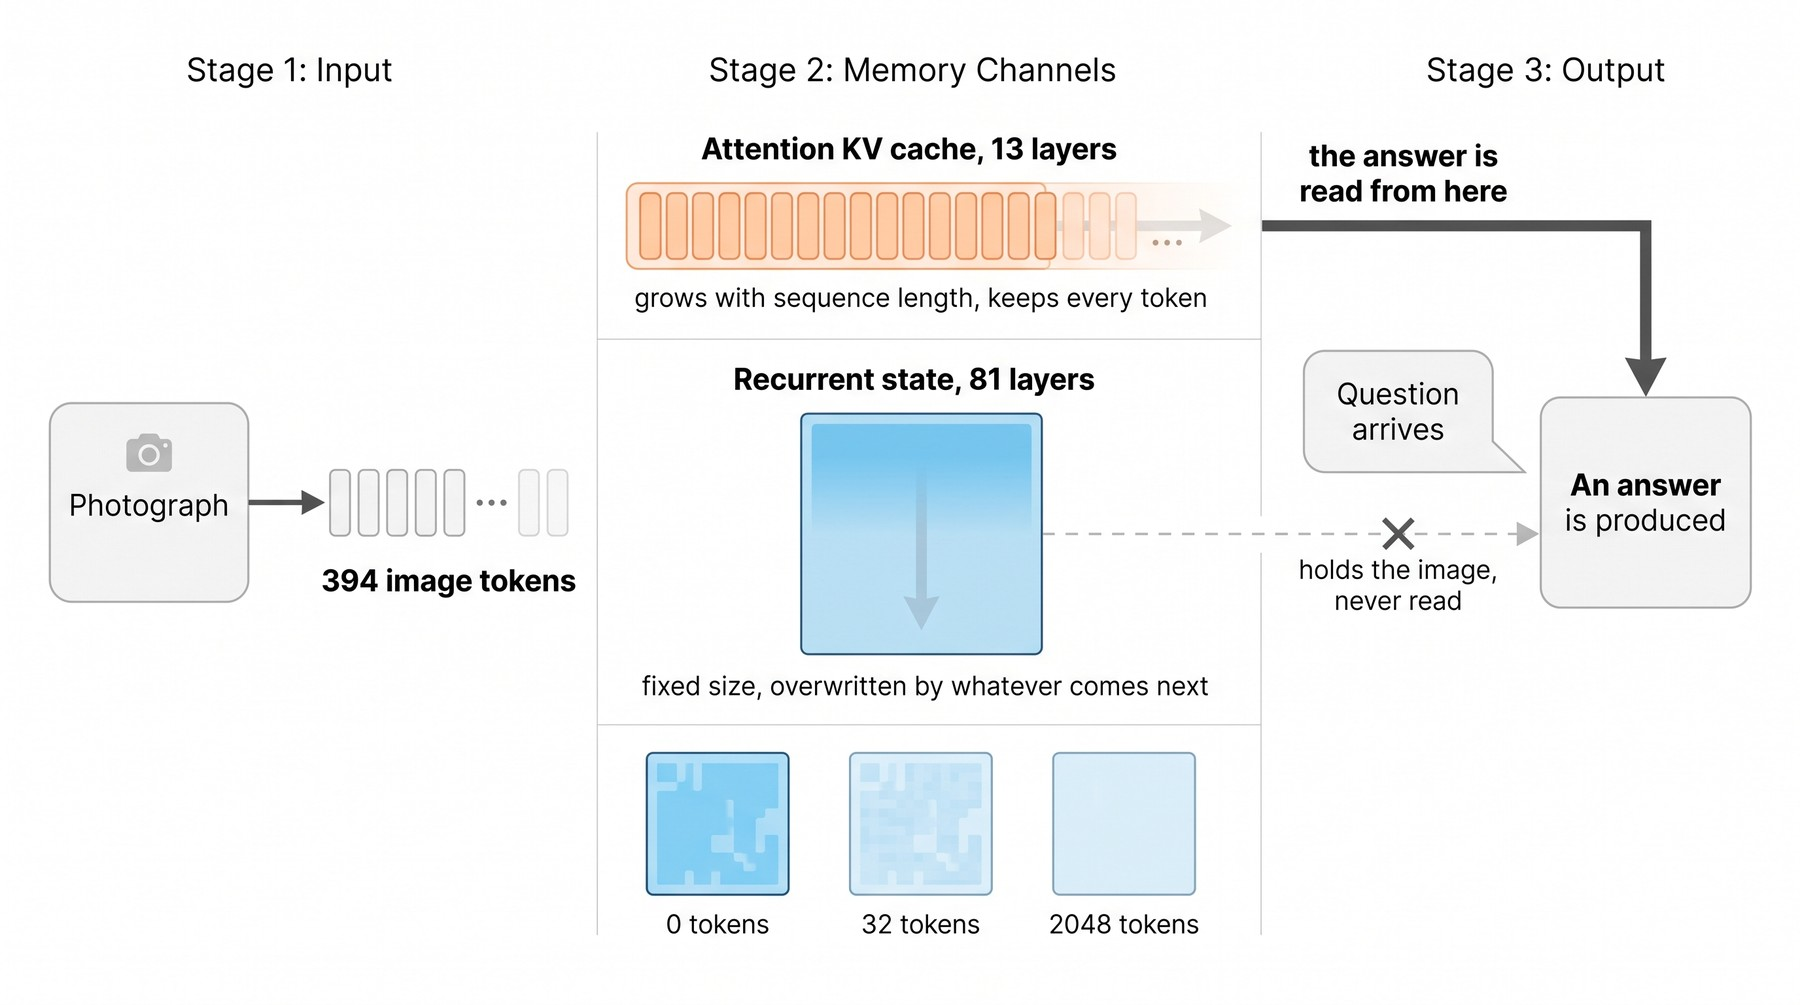
\includegraphics[width=0.94\linewidth]{assets/fig_idea.jpg}
\caption{The two memory channels of a hybrid vision-language model and the
question this paper asks of them.}
\end{figure}

\section{What Was Known Before, and What Is New Here}

Linear-attention and state-space sequence models replace the growing key-value
cache of a transformer with a state of fixed size
\cite{katharopoulos2020linear,gu2022s4,peng2023rwkv,gu2023mamba,dao2024mamba2,beck2024xlstm}.
Because a fixed state cannot grow with the context, most deployed systems keep a
few attention layers alongside it, and the resulting hybrids are now common
\cite{lieber2024jamba,glorioso2024zamba,de2024griffin,ren2025samba,waleffe2024empirical}.
This paper asks what the recurrent half of such a model is actually holding.

The premise that a fixed-size recurrent state must eventually lose information
from context is not ours and we do not claim it. Jelassi et al.\
\cite{jelassi2024copying} prove that transformers can copy exponentially long
strings while generalized state space models are, in their words,
``fundamentally limited by their fixed-size latent state'', and show empirically
that pretrained transformers ``dramatically outperform state space models at
copying and retrieving information from context''. Related results sharpen the
same point from other directions: state-space models are limited to $\mathrm{TC}^0$
and cannot reliably track state \cite{merrill2024illusion}, in-context retrieval
is the specific bottleneck separating recurrent models from transformers
\cite{wen2024rnns}, and most of the quality gap between efficient architectures
and attention is attributable to recall \cite{arora2023zoology,arora2024based}.
Any reader who knows these results should read our work as building on them
rather than rediscovering them.

Table~\ref{tab:novelty} states what that literature establishes and what this
paper adds.

\begin{table}[h]
\centering\small
\begin{tabular}{p{0.44\linewidth}p{0.48\linewidth}}
\toprule
\textbf{Established by prior work} & \textbf{New here} \\
\midrule
A fixed-size state must lose information from context, with a capacity proof
and behavioural evidence \cite{jelassi2024copying,merrill2024illusion,wen2024rnns}.
& \emph{When}. A retention horizon in tokens, computed from the model's own
$A$ and $\Delta$ with nothing fitted, at three scales. \\
\addlinespace
Recurrent models underperform at copying and retrieval as a class
\cite{arora2023zoology,arora2024based}.
& \emph{What survives}. The failure is content-selective: object identity is
highly decodable at the same instant that count and position are near chance. \\
\addlinespace
Architectures are compared to one another from the outside.
& \emph{Causal localisation inside one model}, and the finding that the
recurrent channel relays rather than stores, which makes probing it at distance
a measurement of the attention channel. \\
\addlinespace
Visual tokens and key-value entries carry substantial redundancy that can be
pruned \cite{chen2024fastv,yang2024visionzip,shang2025prumerge}.
& \emph{What underwrites that premise}, and that its safety margin shrinks
with distance from the image on a hybrid. \\
\bottomrule
\end{tabular}
\caption{Delineation of prior work and contribution.}
\label{tab:novelty}
\end{table}

\section{Significance}

Hybrid linear-attention models are being adopted because a fixed-size state
promises constant-memory inference. The design question that follows is which
work the recurrent channel can actually be trusted with. This paper turns that
from a matter of judgement into a calculation: given a checkpoint's $A$ and its
gate statistics, the number of tokens over which its recurrent state retains
what it wrote can be computed before any experiment is run. For Zamba2-VL-7B
that number is single digits, which is far shorter than the intuition invited by
a state of $458{,}752$ numbers per layer.

The consequence for practice is concrete. A substantial line of work accelerates
vision-language models by discarding visual tokens or evicting their key-value
entries, on the stated premise that those entries are largely redundant
\cite{chen2024fastv,yang2024visionzip,shang2025prumerge}, alongside a parallel
line that evicts key-value entries in language models on similar grounds
\cite{zhang2023h2o,li2024snapkv,xiao2024streaming}. Those methods were developed and
validated on dense transformers, where they work, and we find they largely
survive the move to this hybrid: a quarter of the visual entries is enough to
hold accuracy at both distances we tested. What does not survive is the safety
margin. The recurrent channel underwrites that redundancy by relaying the
picture, and it only relays for a few tokens, so the cost of aggressive pruning
roughly doubles between a prompt that asks immediately and one that asks
thirty-two tokens later. A method tuned and validated on short prompts will
therefore look safer than it is, which is the failure mode hardest to catch in
benchmarking.

\section{Model and Instruments}

\subsection{The model}

Zamba2-VL-7B \cite{zamba2vl} is the vision-language member of the Zamba family
\cite{glorioso2024zamba}, which pairs a Mamba2 backbone \cite{dao2024mamba2}
with a shared attention module, and it takes its vision encoder from Qwen2.5-VL
\cite{bai2025qwen25vl}. It is Apache-2.0 licensed and has 81 decoder layers. Every one carries a Mamba2
mixer, and 13 of them additionally carry a shared attention block, at layer
indices 6, 11, 17, 23, 29, 35, 41, 47, 53, 59, 65, 71 and 77. The recurrent
channel therefore spans all 81 layers and the attention channel spans 13. Each
layer's recurrent state is a tensor of shape $[112, 64, 64]$, which is
$458{,}752$ numbers. One image occupies between 345 and 415 tokens depending on
its aspect ratio.

\subsection{Reading the state}

The Mamba2 recurrence is
\begin{equation}
S_t = S_{t-1}\exp(\Delta_t A) + \Delta_t\, x_t B_t^{\top},
\qquad y_t = S_t C_t ,
\end{equation}
so writing uses $(x, B)$, reading uses $C$, and retention of anything already
present is governed by $A$ and $\Delta$ alone. We verified each of these
against the installed model source rather than assuming the canonical form.
In particular $A = -\exp(A_{\log})$ is a per-head scalar, the gate is
$\Delta = \mathrm{softplus}(\Delta_{\text{raw}} + b)$ clamped below at
$0.001$ with no upper clamp, and the decay factor is
$\exp(\Delta_t A)$ elementwise.

Reading a representation with a trained classifier is standard
\cite{alain2016probes}, and so are its known hazards: a probe can succeed
because it is powerful rather than because the information is used, which is why
selectivity against a control task matters \cite{hewitt2019control} and why
probing results are read with care \cite{belinkov2022probing}. We therefore
pair every probe with an intervention, in the tradition of causal mediation
analysis \cite{vig2020causal} and activation patching
\cite{meng2022rome,wang2022ioi,zhang2024patching}, and we follow the
recommendation of that literature to report what the intervention does to
behaviour and not only to the readout \cite{zhang2024patching}.

Because $458{,}752$ numbers per layer is far too wide to probe directly, each
layer's state is passed through a fixed Gaussian random projection to 512
features. A Johnson-Lindenstrauss projection preserves linear separability up to
a controlled distortion, so a linear probe on the projected features is, to that
tolerance, a linear probe on the state. The projection columns are drawn
independently, so the first $k$ columns are themselves a valid $k$-feature
projection.

\subsection{Splicing the channels}

The splice exchanges one memory channel between two runs that saw different
images, leaving the other untouched, and then asks the host's question. Swapping
the recurrent channel replaces all 81 states and convolution buffers; swapping
the attention channel replaces the 13 key and value caches. The host cache is
restored exactly afterwards, so one prefill supports many conditions.

\section{Materials}

Trials are built from COCO val2017 instance annotations \cite{lin2014coco}, the
corpus underlying most visual instruction tuning \cite{liu2023llava}, in
three families: which object is present, how many of a named object are present,
and where in the picture a named object is. All are eight-way forced choice, so
the chance rate is exactly $12.5\%$. Trials are constructed in blocks of eight
that share one identical candidate list, with each candidate correct exactly
once inside the block. That construction is what makes the pre-image control
interpretable: with the candidate set fixed and the answer balanced, a decoder
that has not seen the image cannot exceed chance by exploiting a prior over
candidates.

Images are fetched at native geometry for the decay experiments. For the splice
they are letterboxed onto a common square canvas, because two runs on images of
different shape emit different numbers of vision tokens and therefore
different-length attention caches, which cannot be exchanged. Letterboxing
rather than square resizing matters: in a pilot, a plain square resize deformed
the content enough to halve identity accuracy, so every splice image is
letterboxed.

\section{Result 1: The State Records Gist, Not Particulars}

At the moment of writing, the recurrent state is highly informative about which
object is present and close to uninformative about how many or where. Probing
the full state across all 81 layers reads identity at $83.1\%$ against a
$12.5\%$ chance rate ($p = 6 \times 10^{-92}$, $n = 160$), count at $19.4\%$
($p = 0.009$) and position at $17.5\%$ ($p = 0.041$).

Those figures understate what is linearly present. The full-state feature vector
is $81 \times 512 = 41{,}472$ dimensions, which is heavily overparameterised
relative to the number of trials, and a probe on a single layer does
substantially better. Layer 64 alone reads identity at $92.5\%$, and the last
21 layers (60 to 80) average $85.2\%$, against $59.0\%$ for the middle third of
the stack (layers 27 to 53). On the identical trials the full-state probe reads $71.7\%$. The
gist is therefore both stronger than the aggregate number suggests and localised
in depth, concentrating in the late layers.

\begin{figure}[h]
\centering

\includegraphics[width=\linewidth]{assets/f1_horizon_depth.png}
\caption{\textbf{Left:} identity decoded from the recurrent state against
distance from the image, at three model scales, 120 trials per point. The
pre-image control reads exactly $12.5\%$ at every scale. \textbf{Right:}
identity decoded from each layer's state alone at the instant of writing, with
red marking the 13 layers that also carry attention. A probe given all 81 layers
at once does worse than the best single layer, because $41{,}472$ features on
120 trials is heavily overparameterised.}
\label{fig:horizon}
\end{figure}

\keyfinding{The recurrent state is not a compressed copy of the image. It is a
selective summary that keeps object identity and discards count and position, and
that selection is visible at the instant of writing rather than emerging over
distance.}

\section{Result 2: The Forgetting Horizon, Predicted From the Weights}

\subsection{The prediction}

Retention of whatever the state held, after $k$ further tokens, is
\begin{equation}
R(k) = \exp\!\Big(A \sum_{t=1}^{k}\Delta_t\Big),
\qquad
\text{half-life} = \frac{\ln 2}{|A|\,\bar{\Delta}} .
\end{equation}
$A$ is a stored weight. $\bar{\Delta}$ is measured from the gate channels of the
input projection over the tokens that follow the image, on the same prompts the
decay experiment uses. Nothing here is fitted to a decay curve.

Across all $81 \times 112 = 9{,}072$ heads the predicted median half-life is
$6.6$ tokens, with an interquartile range of $2.8$ to $17.8$. $85.0\%$ of heads
fall below 32 tokens and $0.08\%$ above 512. Measured over eight different
photographs the median moves only between $6.44$ and $6.86$ tokens, so the
horizon is a property of the model rather than of the stimulus.

\subsection{The measurement}

The original collection measured distances $0$ and then $32$, which is far
outside the region where the prediction is specific. Table~\ref{tab:fine} shows
a finer sweep on 120 identity trials.

\begin{table}[h]
\centering\small
\begin{tabular}{rrrrr}
\toprule
tokens & probe accuracy & $p$ & behaviour & predicted retention (median) \\
\midrule
0  & $71.7\%$ & $2\times10^{-50}$ & $94.2\%$ & $1.000$ \\
1  & $60.0\%$ & $2\times10^{-34}$ & $96.7\%$ & $0.901$ \\
2  & $59.2\%$ & $2\times10^{-33}$ & $97.5\%$ & $0.812$ \\
4  & $41.7\%$ & $1\times10^{-15}$ & $96.7\%$ & $0.659$ \\
8  & $35.0\%$ & $2\times10^{-10}$ & $97.5\%$ & $0.434$ \\
12 & $30.0\%$ & $3\times10^{-7}$  & $96.7\%$ & $0.286$ \\
16 & $24.2\%$ & $3\times10^{-4}$  & $97.5\%$ & $0.188$ \\
24 & $29.2\%$ & $1\times10^{-6}$  & $95.8\%$ & $0.082$ \\
32 & $20.8\%$ & $7\times10^{-3}$  & $95.0\%$ & $0.036$ \\
48 & $25.8\%$ & $6\times10^{-5}$  & $97.5\%$ & $0.007$ \\
64 & $21.7\%$ & $3\times10^{-3}$  & $98.3\%$ & $0.001$ \\
\bottomrule
\end{tabular}
\caption{Decodability of object identity against distance from the image, on
120 trials at every distance, with the retention predicted from the weights
alongside. Chance is $12.5\%$. The pre-image control reads exactly $12.5\%$.}
\label{tab:fine}
\end{table}

The above-chance signal halves at $4.0$ tokens, inside the predicted
interquartile range of $2.8$ to $17.8$. Normalised to its value at distance
zero, measured decodability correlates with predicted mean retention at
$r = 0.973$ across the eleven distances, with no free parameters. Beyond 16
tokens the measured curve sits above the predicted median and between the median
and the mean, which is what the heavy tail of slow heads predicts: the residual
signal at long distance is carried by the minority of heads with long
half-lives.



Throughout this collapse the model's own accuracy never moves. It answers
correctly on $94$ to $98\%$ of trials at every distance, including those where
the state has been emptied.

\subsection{The within-model test, which inverts the prediction}

A curve comparison cannot rule out coincidence, so we split the heads into
thirds by predicted half-life and probed each third separately, using the same
projection basis so the strata are comparable to one another and to the
unstratified probe. The thirds have predicted median half-lives of $2.0$, $6.6$
and $29.0$ tokens, a fourteen-fold span. Decay predicts that the slow third
stays decodable furthest.

The opposite happened. Table~\ref{tab:strata} shows the fast third, whose
predicted half-life is two tokens, decoding object identity at $61.7\%$ after
sixty-four tokens, while the slow third falls to $16.7\%$ over the same span.

\begin{table}[h]
\centering\small
\begin{tabular}{lrrrrr}
\toprule
stratum & predicted $t_{1/2}$ & $d{=}0$ & $d{=}16$ & $d{=}64$ & signal kept at $d{=}64$ \\
\midrule
fast   & $2.0$  & $87.5\%$ & $73.3\%$ & $61.7\%$ & $0.66$ \\
middle & $6.6$  & $81.7\%$ & $20.8\%$ & $15.0\%$ & $0.04$ \\
slow   & $29.0$ & $68.3\%$ & $17.5\%$ & $16.7\%$ & $0.08$ \\
\bottomrule
\end{tabular}
\caption{Identity decodability by head stratum. ``Signal kept'' is the
above-chance excess at $d{=}64$ as a fraction of the excess at $d{=}0$. The
ordering is the reverse of the decay prediction.}
\label{tab:strata}
\end{table}

\begin{figure}[h]
\centering
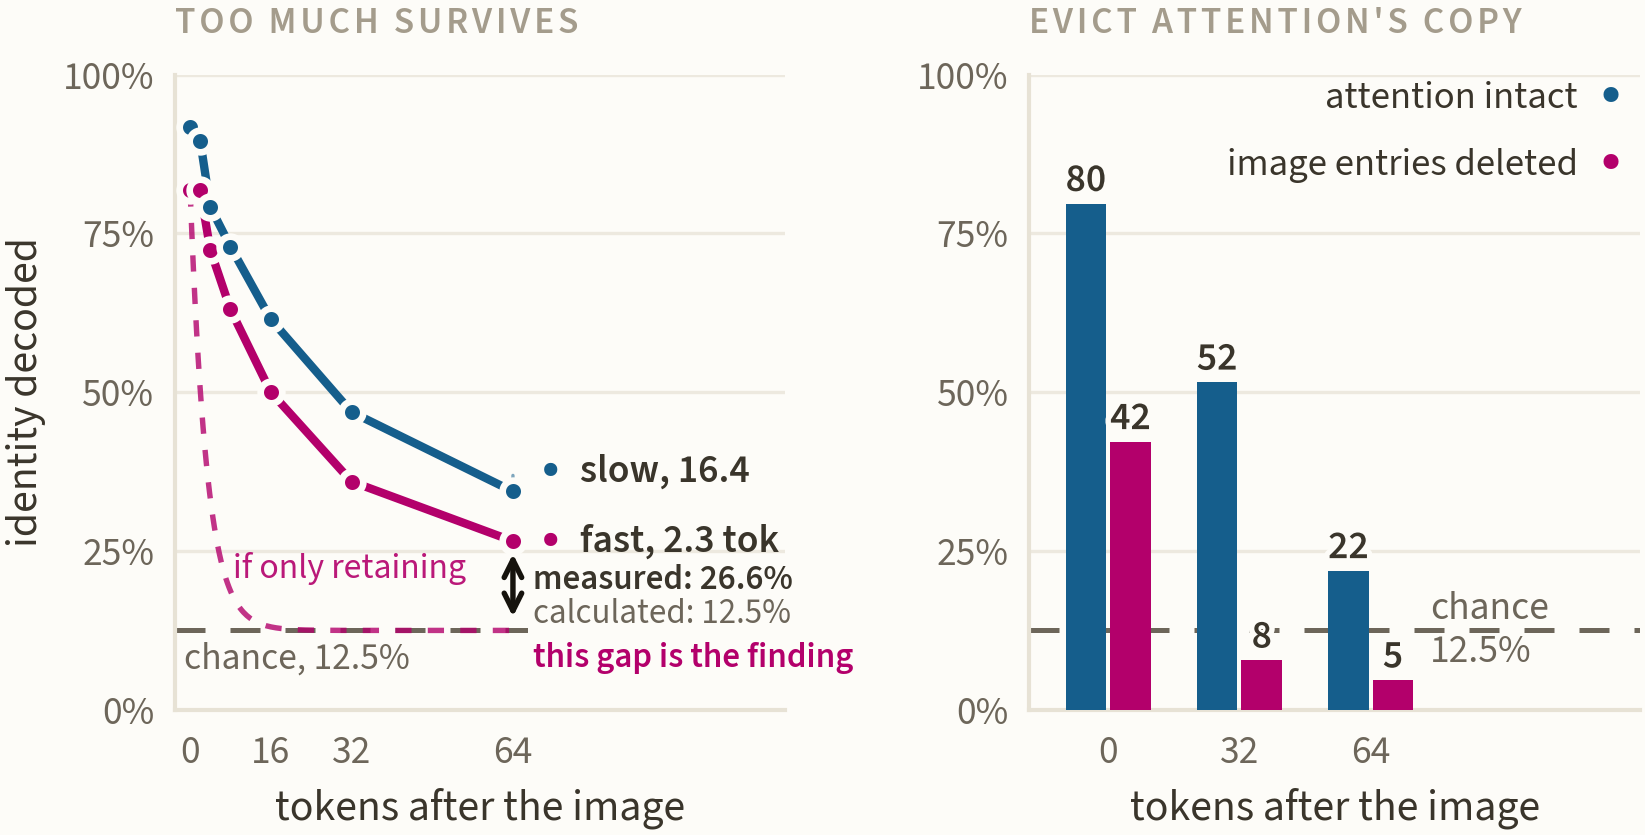
\includegraphics[width=\linewidth]{assets/f2_relay.png}
\caption{\textbf{Left:} heads split into thirds by the half-life implied by
their own $A$ and gate, labelled with each third's predicted median. Decay
predicts the slow third survives longest; the measured ordering is the reverse.
\textbf{Right:} the same recurrent state probed with and without the attention
channel's copy of the image, fast heads only, $n = 64$ per bar. The eviction
happens immediately after the image is read and never touches the recurrent
state, which is identical in both runs at that instant.}
\label{fig:relay}
\end{figure}

The obvious confound runs the wrong way. Because the split is global rather than
within-layer, the strata draw unequal numbers of heads from each layer, and
depth matters a great deal for decoding. But the fast stratum is concentrated in
\emph{earlier} layers (mean layer $32.2$, against $45.5$ for the middle
stratum), with only $10.1\%$ of its mass in the strong late layers against
$37.5\%$ for the middle stratum, and a depth-weighted per-layer accuracy of
$0.653$ against $0.729$. It sits in worse layers and still wins.

\keyfinding{A head with a two-token half-life cannot be holding something
written sixty-four tokens earlier: by then its state is composed almost entirely
of recent writes. If such a head decodes object identity at $61.7\%$, the
identity information in its state arrived recently, which means something else
in the model is still supplying it.}

\section{Result 3: The Recurrent Channel Is a Relay, Not a Store}

The only component that still holds the image at distance is the attention
channel, whose key-value entries are untouched by distance. We tested that
directly. Each trial was run twice, identically, except that in one run the
visual key-value entries were evicted from all 13 attention layers immediately
after the image was read and \emph{before a single filler token was processed}.
The eviction does not touch the recurrent state, which at that instant is
identical in both runs.

If the state is remembering, eviction should not change what a probe reads from
it. If the state is a relay, eviction should collapse decodability at distance,
and should do so most severely for the fast heads.

\begin{table}[h]
\centering\small
\begin{tabular}{lrrrr}
\toprule
stratum & distance & visual KV intact & visual KV evicted & change \\
\midrule
fast   & 0  & $79.7\%$ & $42.2\%$ & $-37.5$ \\
fast   & 32 & $51.6\%$ & $\mathbf{7.8\%}$  & $-43.7$ \\
fast   & 64 & $21.9\%$ & $4.7\%$  & $-17.2$ \\
\addlinespace
middle & 0  & $62.5\%$ & $43.8\%$ & $-18.8$ \\
slow   & 0  & $62.5\%$ & $54.7\%$ & $-7.8$  \\
\addlinespace
all    & 0  & $59.4\%$ & $59.4\%$ & $0.0$   \\
all    & 32 & $6.2\%$  & $6.2\%$  & $0.0$   \\
\bottomrule
\end{tabular}
\caption{Identity decodability from the recurrent state with and without the
attention channel's copy of the image, $n = 64$ per cell. Chance is $12.5\%$.
The fast heads' apparent memory at 32 tokens is entirely dependent on the
attention channel: removing it drops them from $51.6\%$ to below chance.}
\label{tab:relay}
\end{table}

\begin{figure}[h]
\centering

\includegraphics[width=\linewidth]{assets/f3_controls.png}
\caption{\textbf{Left:} the control that rules out the perturbation account.
Both interventions remove the same number of positions from the same 13 caches,
one taking the image and the other an equal count of the most recent pre-image
text. They move the readout in opposite directions. \textbf{Right:} accuracy
lost when the visual entries are zeroed at all 13 attention layers, at only the
earliest three, and at only the latest three. The earliest three reproduce most
of the full effect; the latest three do nothing.}
\label{fig:controls}
\end{figure}

\subsection{Controls: the eviction removes the image, not merely positions}
\label{sec:controls}

The standing objection to the eviction contrast is that it changes more than the
image's presence. Removing the visual entries shortens every attention cache by
roughly 400 positions and changes the softmax normalisation for every token that
follows. The matched control is to remove an equal number of \emph{non-visual}
positions from the same caches, and we ran it on ten strata formed by deciles of
predicted half-life rather than thirds, with 64 trials per cell
(Table~\ref{tab:controls}).

The two interventions move the readout in opposite directions. At 32 tokens,
evicting the image costs the fastest decile $18.8$ points while evicting an
equal number of the most recent pre-image text positions \emph{raises} it by
$29.7$ points; averaged over the ten strata the two effects are $-6.4$ and
$+12.5$ points. Removing text plausibly helps because it removes content
competing with the image for the residual stream. A perturbation account
predicts the same sign for both interventions, so this double dissociation rules
it out.

\begin{table}[h]
\centering\small
\begin{tabular}{rrrrrrr}
\toprule
& & \multicolumn{3}{c}{$d = 0$} & \multicolumn{2}{c}{$d = 32$} \\
\cmidrule(lr){3-5}\cmidrule(lr){6-7}
decile & pred.\ $t_{1/2}$ & intact & evict image & evict text & intact & evict image \\
\midrule
1  & $0.70$ & $56.2\%$ & $18.8\%$ & $78.1\%$ & $31.2\%$ & $12.5\%$ \\
2  & $1.84$ & $56.2\%$ & $17.2\%$ & $79.7\%$ & $29.7\%$ & $12.5\%$ \\
3  & $2.75$ & $53.1\%$ & $18.8\%$ & $73.4\%$ & $20.3\%$ & $4.7\%$  \\
4  & $3.79$ & $46.9\%$ & $21.9\%$ & $71.9\%$ & $23.4\%$ & $15.6\%$ \\
5  & $5.38$ & $31.2\%$ & $26.6\%$ & $42.2\%$ & $12.5\%$ & $9.4\%$  \\
6  & $8.15$ & $35.9\%$ & $40.6\%$ & $51.6\%$ & $17.2\%$ & $20.3\%$ \\
7  & $11.8$ & $37.5\%$ & $25.0\%$ & $54.7\%$ & $10.9\%$ & $9.4\%$  \\
8  & $17.8$ & $45.3\%$ & $29.7\%$ & $57.8\%$ & $20.3\%$ & $18.8\%$ \\
9  & $32.0$ & $28.1\%$ & $26.6\%$ & $32.8\%$ & $15.6\%$ & $15.6\%$ \\
10 & $73.3$ & $51.6\%$ & $29.7\%$ & $46.9\%$ & $23.4\%$ & $21.9\%$ \\
\bottomrule
\end{tabular}
\caption{The matched-eviction control by decile of predicted half-life, $n = 64$
per cell, chance $12.5\%$. ``Evict image'' and ``evict text'' delete the same
number of positions from the same 13 attention caches. Single cells carry about
$6$ points of binomial noise at $n = 64$, and two of the twenty image-eviction
cells fall slightly the wrong way; the trend rather than any one cell is the
result. The drop under image eviction correlates with the decay rate
$1/t_{1/2}$ at $r = 0.647$ at $d{=}0$ and $r = 0.800$ at $d{=}32$.}
\label{tab:controls}
\end{table}

The same collection locates where the relay enters. Zeroing the visual entries
at only the three earliest attention layers reproduces $15.8$ of the $17.2$
points lost when all thirteen are zeroed, while the three latest layers produce
$0.5$ points. Visual information enters early and is consumed downstream. For
per-layer conditions we zero rather than delete, because Zamba2's attention
blocks are shared and take a single mask length; the two operations agree to
$2.34$ points at $d{=}32$ where both are available, which is the validation of
that substitution.

Finally, the contrast is stable across the choice of projection basis. Repeating
it with three independent Gaussian projections gives, for the fast stratum at
$32$ tokens, intact $31.2 \pm 1.6\%$ against evicted $9.9 \pm 1.8\%$ (mean and
standard deviation over seeds), while the slow stratum shows no eviction effect
at any seed.

\subsection{The decay parameters predict how much is relayed}

Result 2 found that the parameter-derived horizon does not predict the measured
decodability curve. It does predict something else, and the quantity it predicts
is the one the relay account says it should. A head that forgets quickly must
depend more heavily on fresh re-encoding, so its readout should be hurt more by
removing the source of that re-encoding. Ordering the strata by decay rate gives
exactly that:

\begin{table}[h]
\centering\small
\begin{tabular}{lrrr}
\toprule
stratum & predicted half-life & decay rate $1/t_{1/2}$ & drop under eviction at $d{=}0$ \\
\midrule
fast   & $1.98$  & $0.505$ & $37.5$ points \\
middle & $6.64$  & $0.151$ & $18.8$ points \\
slow   & $28.96$ & $0.035$ & $7.8$ points \\
\bottomrule
\end{tabular}
\caption{Dependence on the attention channel, against the decay rate implied by
each stratum's own $A$ and gate. The two quantities correlate at $r = 0.991$.}
\label{tab:dose}
\end{table}

The decay calculation therefore does carry predictive content, but about the
mechanism rather than about the curve: it says which heads are relaying and
which are retaining. With three strata this is suggestive rather than
established, and we flag it as such in the limitations.

The pattern is exactly the relay prediction and it is not subtle. At 32 tokens
the fast heads read $51.6\%$ with the attention channel intact and $7.8\%$
without it, which is below the $12.5\%$ chance rate. Thirty-three correct
predictions out of sixty-four become five. Meanwhile the slow heads at distance
zero, whose content was written while the image was being read, are barely
affected by eviction at all ($62.5\%$ to $54.7\%$), which is the control that
shows the intervention is not simply breaking the model.

\keyfinding{What a probe reads out of the recurrent state at distance is not
what the state remembered. It is what the attention channel is still supplying,
re-encoded afresh at every token. The recurrent channel relays the picture; it
does not store it.}

\subsection{What the probe can see, and why that matters here}
\label{sec:sensitivity}

The obvious objection to the eviction contrast is that the probe may simply be
insensitive to weak signals. Freshly re-encoded content plausibly sits at higher
amplitude than content written long ago and decayed, so a probe that finds
strong signals and misses faint ones would produce these observations without
the state having stopped storing anything.

That objection is quantitative and can be measured. Taking the distance-zero
features, where the image is present at full strength, we attenuate each trial's
own contribution while substituting an equal amount of unrelated variation from
another trial, holding total variance roughly constant:
$x_i(\alpha) = \mu + \alpha (x_i - \mu) + \sqrt{1-\alpha^2}\,(x_j - \mu)$.
This is what decay followed by overwriting does to a stored trace.

The probe loses half its signal at $\alpha = 0.78$ and is indistinguishable from
chance by $\alpha \approx 0.25$. The best single-layer probe behaves the same
way, halving at $\alpha = 0.75$. So this instrument cannot see content below
roughly a quarter of full amplitude.

That number does the work. The weights predict retention at thirty-two tokens of
$3.7\%$ at the median and $18\%$ at the mean, both below the floor. Retained
content at that distance therefore \emph{could not} produce a visible reading.
Yet the intact probe reads the fast heads at $51.6\%$ there. Whatever it is
reading cannot be a retained trace, because a retained trace at that distance is
invisible to it. It must be high in amplitude, which means recently written. And
removing the attention channel's copy removes it.

\begin{figure}[h]
\centering
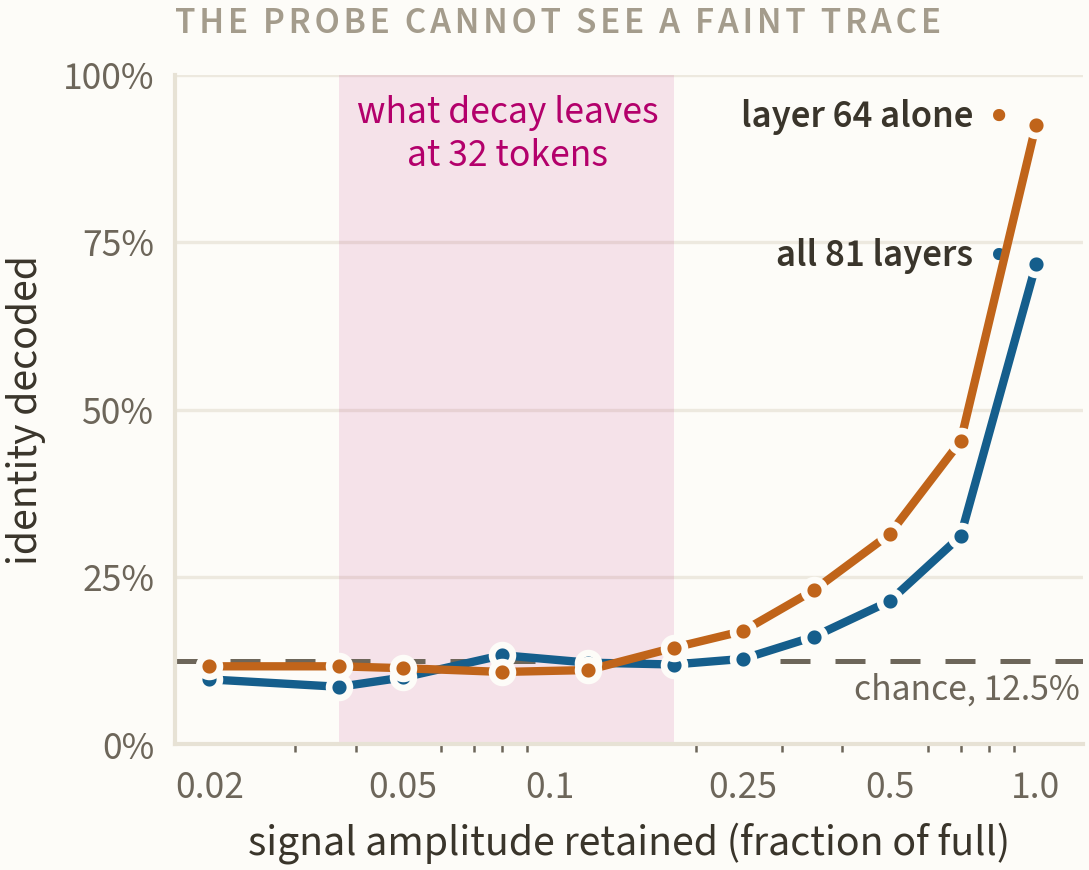
\includegraphics[width=0.72\linewidth]{assets/f4_sensitivity.png}
\caption{How faint a signal the probe can still recover. Each trial's own
contribution is attenuated while an equal amount of unrelated variation is
substituted, holding total variance roughly constant. The shaded band is what
the model's decay parameters leave of a stored trace after 32 tokens, between
the median and the mean over heads. Both probes are at chance throughout that
band, so a visible reading at 32 tokens cannot be a retained one.}
\label{fig:sensitivity}
\end{figure}

\keyfinding{The probe's insensitivity to faint signals is what makes the
positive reading informative. A signal the instrument can see at thirty-two
tokens is necessarily a fresh one, because a retained one would be four to six
times below its detection floor.}

The same measurement bounds what we may conclude. Whether faint retained content
persists below the floor is not answerable with this instrument at any distance
beyond a few tokens, so this paper does not claim the state stops storing the
image. It claims that what a probe reads at distance is not retention, and that
it depends causally on the attention channel.

This resolves three things at once. It explains why the measured horizon exceeds
the predicted one, and why the gap grows in smaller models: the probe has never
been measuring retention. It explains why the fast heads appeared to retain
most, since they track the residual stream most closely and the residual stream
is where the re-supplied information arrives. And it supplies the mechanism behind the
causal result, which the next section takes up.

\section{Result 4: Causally, the Answer Follows the Attention Channel}

The splice exchanges one memory channel between two runs that saw different
images and then asks the host's question. Pairs are admitted only if the host
and the donor each answer their own question correctly, so the ceiling is
$100\%$ by construction. Of 111 attempted pairs, 11 were rejected on that
criterion and none were rejected for mismatched cache length. Every recurrent
swap was verified to have changed the state, 100 of 100.

\begin{table}[h]
\centering\small
\begin{tabular}{lrrr}
\toprule
condition & layers swapped & follows host & follows donor \\
\midrule
no swap                       & 0  & $100/100$ $[96,100]$ & $0/100$ $[0,4]$ \\
recurrent, all 81 states      & 0  & $100/100$ $[96,100]$ & $0/100$ $[0,4]$ \\
\addlinespace
attention, 1 layer            & 1  & $100/100$ $[96,100]$ & $0/100$ $[0,4]$ \\
attention, 3 layers spread    & 3  & $98/100$ $[93,99]$   & $0/100$ $[0,4]$ \\
attention, 7 layers           & 7  & $4/100$ $[2,10]$     & $94/100$ $[88,97]$ \\
attention, all 13             & 13 & $0/100$ $[0,4]$      & $98/100$ $[93,99]$ \\
\addlinespace
attention, earliest 3         & 3  & $94/100$ $[88,97]$   & $1/100$ $[0,5]$ \\
attention, latest 3           & 3  & $100/100$ $[96,100]$ & $0/100$ $[0,4]$ \\
both channels                 & 13 & $0/100$ $[0,4]$      & $100/100$ $[96,100]$ \\
\bottomrule
\end{tabular}
\caption{The splice at 100 pairs with a $100\%$ ceiling. Brackets are $95\%$
Wilson intervals in percent. Replacing the entire recurrent memory of all 81
layers changes nothing; replacing seven of the thirteen attention caches flips
the answer to the other image.}
\label{tab:splice}
\end{table}

\begin{figure}[h]
\centering
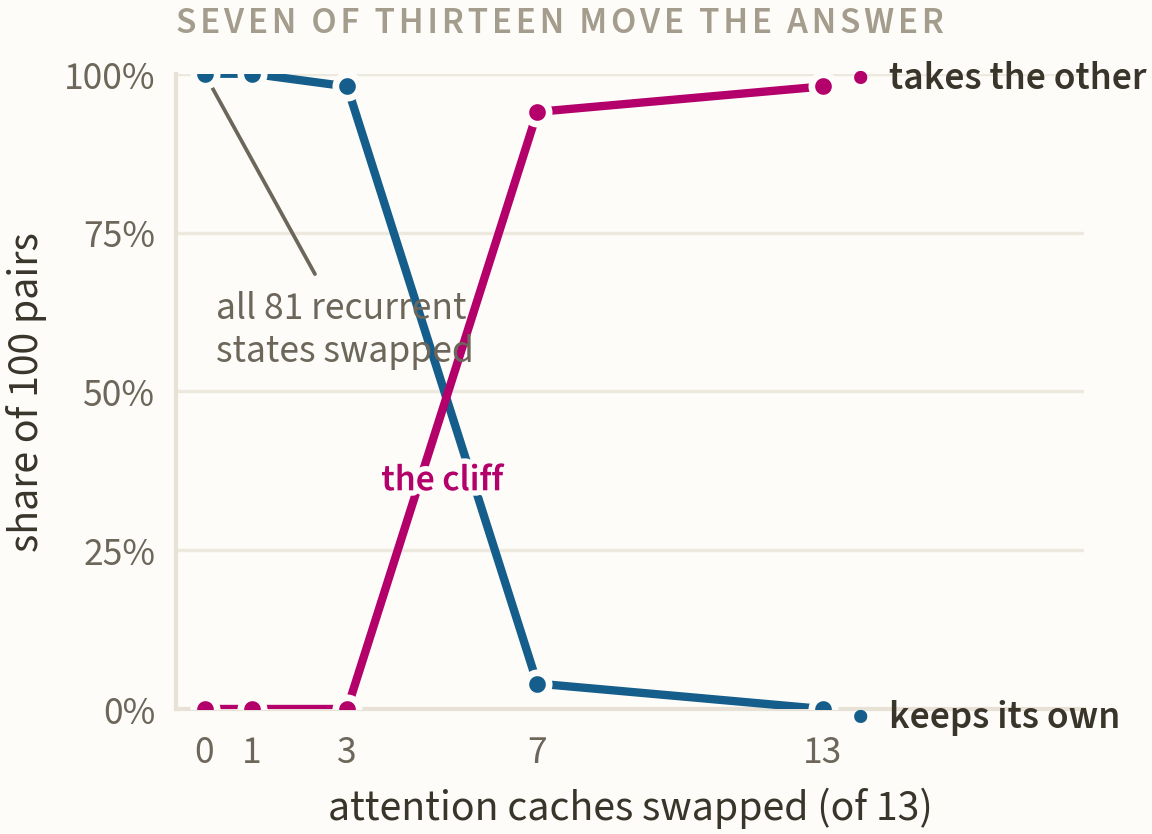
\includegraphics[width=0.72\linewidth]{assets/f5_splice.png}
\caption{How many of the thirteen attention caches must be exchanged before the
answer follows the other image, over 100 pairs in which both images were
answered correctly beforehand. The leftmost point is the recurrent swap: all 81
states replaced, no attention cache touched, no effect.}
\label{fig:splice}
\end{figure}

Three readings. First, the recurrent null is now complete rather than
approximate: exchanging all 81 recurrent states and convolution buffers leaves
$100$ of $100$ answers following the host's own image, with every swap verified
to have taken effect. Second, the attention channel is causally sufficient:
swapping seven of the thirteen caches moves $94$ of $100$ answers to the donor's
image. Third, and new, the dependence is graded and distributed. One attention
layer does nothing, three spread across the stack move two answers, seven move
almost all of them. No small subset suffices, so the picture is held across the
attention layers rather than concentrated in a few. The earliest three layers
have a small effect where the latest three have none, which is consistent with
visual information entering early and being consumed downstream.

Read with Result 3, the recurrent null stops being a puzzle. Replacing the
recurrent state cannot change the answer because the replacement is erased
within a few tokens and rewritten from the attention channel, which the recurrent
swap leaves untouched. The two results are the same fact seen from two sides.
\section{Result 5: Scale, and Where the Prediction Fails}

The instruments read every shape from the loaded model's configuration rather
than assuming Zamba2-VL-7B's, which is necessary rather than tidy: the 2.7B and
1.2B checkpoints use a single B/C group where the 7B uses two, and the 1.2B
carries a state dimension of 128 where the others carry 64. Table~\ref{tab:scale}
reports the same protocol at all three scales.

\begin{table}[h]
\centering\small
\begin{tabular}{lrrrrrr}
\toprule
model & layers & attn & probe $d{=}0$ & probe $d{=}64$ & measured $t_{1/2}$ & predicted $t_{1/2}$ \\
\midrule
Zamba2-VL-7B   & 81 & 13 & $71.7\%$ & $21.7\%$ & $4.0$  & $6.64$ \\
Zamba2-VL-2.7B & 54 &  9 & $84.2\%$ & $31.7\%$ & $9.6$  & $2.91$ \\
Zamba2-VL-1.2B & 38 &  6 & $83.3\%$ & $34.2\%$ & $14.3$ & $2.58$ \\
\bottomrule
\end{tabular}
\caption{The same protocol at three scales, 120 identity trials per distance.
The pre-image control reads exactly $12.5\%$ at every scale. Half-lives are in
tokens: measured is the distance at which above-chance decodability halves,
predicted is the median over heads of $\ln 2/(|A|\bar{\Delta})$.}
\label{tab:scale}
\end{table}

Two things follow, and the second is a negative result we report rather than
bury.

The parameter-derived horizon is short at every scale. Median predicted
half-lives are $6.64$, $2.91$ and $2.58$ tokens, and the fraction of heads with
a predicted half-life under 32 tokens is $85.0\%$, $97.9\%$ and $95.6\%$. Whatever
the recurrent state genuinely retains of its own past, it retains for single-digit
token counts in all three models.

But the predicted horizon does not predict the measured one. Across the three
models the two quantities move in opposite directions: prediction falls with
scale while measurement rises. On the 7B alone the agreement looked strong, with
measured decodability tracking predicted retention at $r = 0.973$ across eleven
distances. That agreement does not replicate, and we therefore do not claim
that the decay calculation explains the measured decay curve. The next section
shows why it cannot, and what the probe is actually reading at distance.

\section{Result 6: Visual Key-Value Eviction Removes the Only Copy, Eventually}

The redundancy premise behind visual token and key-value pruning can be tested
directly. We evict a fraction of the visual key-value entries from all 13
attention layers immediately after the image is read, then let the filler and
the question stream past the pruned cache, and measure the model's own
accuracy. Retention $\rho$ is the fraction of visual positions kept, sampled
uniformly, and the question is asked $d$ tokens after the image.

\begin{table}[h]
\centering\small
\begin{tabular}{lrrrr}
\toprule
visual KV retained & $d{=}0$ & $d{=}32$ & $d{=}128$ & $d{=}512$ \\
\midrule
$100\%$ & $97.9\%$ & $95.8\%$ & $100.0\%$ & $97.9\%$ \\
$25\%$  & $91.7\%$ & $95.8\%$ & $95.8\%$  & $91.7\%$ \\
$5\%$   & $87.5\%$ & $77.1\%$ & $75.0\%$  & $64.6\%$ \\
$0\%$   & $64.6\%$ & $37.5\%$ & $31.2\%$  & $22.9\%$ \\
\bottomrule
\end{tabular}
\caption{Behavioural accuracy under visual key-value eviction, against distance
between the image and the question. $n = 48$ per cell, chance $12.5\%$, no
failures. The unpruned row is flat, so distance alone costs nothing.}
\label{tab:eviction}
\end{table}

Read as cost relative to the unpruned baseline at the same distance, the
structure is a clean interaction:

\begin{table}[h]
\centering\small
\begin{tabular}{lrrrr}
\toprule
visual KV retained & $d{=}0$ & $d{=}32$ & $d{=}128$ & $d{=}512$ \\
\midrule
$25\%$ & $6.2$  & $0.0$  & $4.2$  & $6.2$ \\
$5\%$  & $10.4$ & $18.8$ & $25.0$ & $33.3$ \\
$0\%$  & $33.3$ & $58.3$ & $68.8$ & $75.0$ \\
\bottomrule
\end{tabular}
\caption{Accuracy points lost to pruning, relative to the unpruned baseline at
the same distance.}
\label{tab:eviction_cost}
\end{table}

At a quarter of the entries retained there is no distance effect at all: the
cost is $6.2$, $0.0$, $4.2$ and $6.2$ points, which is flat within noise. The
redundancy premise holds on this architecture at that level, and we found no
evidence against it.

Below that level distance begins to matter, and it matters a great deal. At a
twentieth retained the cost triples across the range, from $10.4$ points beside
the image to $33.3$ points at 512 tokens. With every visual entry removed it
runs from $33.3$ to $75.0$. The unpruned row is flat across the same distances,
so this is not a difficulty that grows with prompt length; it is a difficulty
that grows with prompt length \emph{only once the visual entries are gone}.

\begin{figure}[h]
\centering

\includegraphics[width=0.72\linewidth]{assets/f6_eviction.png}
\caption{Model accuracy under visual key-value eviction, against how far the
question sits from the image, $n = 48$ per point. The unpruned line is flat, so
distance alone costs nothing. Keeping a quarter of the entries is also flat.
Below that the lines fan out: the cost of pruning grows with distance only once
the recurrent channel has stopped relaying the picture.}
\label{fig:eviction}
\end{figure}

\keyfinding{There is a retention threshold, somewhere between a quarter and a
twentieth on this model, below which the cost of pruning stops being a fixed
overhead and starts growing with how far the question sits from the image. A
method validated at short range will understate its cost at long range by a
factor of three at $5\%$ retention.}

The zero-retention row is also the cleanest available measure of what the
recurrent channel contributes on its own. With no visual entries anywhere in
the attention caches, accuracy falls from $64.6\%$ beside the image to $22.9\%$
at 512 tokens. That decline is the recurrent channel's contribution decaying,
measured behaviourally and with an instrument entirely independent of the
probe, and it agrees with the picture the probe gives.

There is a discrepancy worth stating plainly rather than smoothing over. At
zero retention the model still answers at $37.5\%$ at thirty-two tokens, well
above the $12.5\%$ chance rate, while our linear probe reads the recurrent
state at close to chance at that distance. The model is using something in the
recurrent channel that the probe does not recover. The probe is a lower bound
on what the state carries, not a measure of it, and the sentence ``the state is
empty'' is not one this evidence supports.

\section{Limitations}

We separate three kinds of limitation: alternative explanations our evidence
does not exclude, limits on what the instruments can see, and limits on scope.
The first kind is the one that should decide how much weight a reader puts on
the central claim, so it comes first.

\subsection{Alternative explanations we have not excluded}

\textbf{Eviction changes more than the image's presence, though the matched
control now argues against it.} Removing the visual key-value entries shortens
every attention layer's cache by roughly 400 positions and changes the softmax
normalisation for every token that follows. Section~\ref{sec:controls} reports
the matched control, evicting an equal number of \emph{non-visual} positions
from the same caches, and finds the two interventions move the readout in
opposite directions, which a pure perturbation cannot produce. What remains
unexcluded is narrower: the pre-image text we remove is not interchangeable with
the image in what it contributes to the residual stream, so the comparison
bounds the perturbation account rather than eliminating every version of it.

\textbf{The relay result could be a sensitivity asymmetry, now bounded but not
eliminated.} Our own data show the probe is a lower bound (below), and a lower
bound need not be a uniform one: freshly re-encoded content plausibly sits at
higher amplitude than content written many tokens earlier and decayed. If the
probe recovers high-amplitude content easily and low-amplitude content poorly,
removing the re-encoded copy would collapse the readout even in a state still
genuinely retaining something. The amplitude calibration of
Section~\ref{sec:sensitivity} answers this by measuring the detection floor and
showing that predicted retention at thirty-two tokens sits below it, so a
visible reading there cannot be a retained one. That argument assumes decay
followed by overwriting acts on the discriminative component roughly as our
attenuation does. A model with no attention channel to relay from would settle
it without that assumption, and we have not tested one.

\textbf{The route is located but not traced.} The layerwise eviction of
Section~\ref{sec:controls} shows the relay enters early: zeroing the three
earliest attention layers reproduces $15.8$ of the $17.2$ points lost when all
thirteen are zeroed, while the three latest produce $0.5$. What is not traced is
the intermediate path, from attention output through the residual stream into a
downstream mixer's write.

\subsection{What the instruments can and cannot see}

\textbf{The probe is a lower bound, and our own behavioural data prove it.}
With every visual key-value entry removed, the model answers at $37.5\%$ at
thirty-two tokens while the probe reads the recurrent state near chance at the
same distance. Something usable survives there that a 512-dimensional random
projection, read by a linear probe trained on 120 examples, does not recover.
Every statement in this paper about what the state contains should be read as a
statement about what is linearly decodable under that instrument. This paper does
not establish that the state is empty of the image at any distance, and makes no
such claim.

\textbf{Probe accuracy depends on the feature-to-trial ratio.} Count read at
chance with 128 projection features and reached $19.4\%$ at 512. In the other
direction, the full $41{,}472$-dimensional state probe reads $71.7\%$ where a
single layer's 512 features read $92.5\%$ on identical trials. Absolute
accuracies are therefore not comparable across collections of different size or
width, and we report them only within a collection. The decay curve in
Table~\ref{tab:fine} is internally consistent because the same 120 trials appear
at every distance.

\textbf{One projection basis for most results.} The eviction contrast was
repeated across three independent Gaussian projection bases and is stable under
them (fast stratum at $d{=}32$: intact $31.2 \pm 1.6\%$ against evicted
$9.9 \pm 1.8\%$, mean and standard deviation over seeds). The decay-curve
collections still use a single fixed basis, so the variance attributable to the
choice of basis is unmeasured there.

\textbf{The stratum dose-response is measured on ten strata, in one model.}
With three thirds the eviction sensitivity is ordered exactly by predicted decay
rate ($37.5$, $18.8$ and $7.8$ points, $r = 0.991$), which on three points is
suggestive rather than established. Repeating it on deciles of predicted
half-life gives $r = 0.800$ at $32$ tokens and $r = 0.647$ at distance zero over
ten strata, with about $6$ points of binomial noise per cell at $n = 64$. The
relationship therefore survives finer stratification, but it is measured on one
model and one task.

\subsection{Scope}

\textbf{One model family, and a second family we tried and failed on.} Results
come from three Zamba2-VL checkpoints, which is one vendor, one architecture
family and one training recipe. This is the principal limit on the paper's
generality and we do not argue around it.

We attempted to extend the relay result to a second family and report the
attempt because its failure is informative. Granite 4.0 h-tiny \cite{granite4} is a Mamba2
hybrid from a different lineage, with 36 recurrent layers to 4 attention layers
against Zamba2-VL-7B's 81 to 13. Its decay parameters read out cleanly and give
a median predicted half-life of $8.7$ tokens, so the horizon calculation of
Section 5 transfers to a second family. The relay contrast does not, for an
instrumental reason: on a code-word recall task the model answers correctly on
$100\%$, $96.9\%$ and $100\%$ of trials at $0$, $32$ and $64$ tokens, and yet a
probe on its recurrent state reads at chance at distance zero. Scaling to 256
trials did not change this ($13.7\%$ against a $12.5\%$ chance rate,
$p = 0.31$), and neither did probing single layers, where the best of 36 layers
reached $19.9\%$.

We suspected the item was too small to write a detectable trace, a one-token
code word against a 345-token image, and tested that by repeating the carrier
sixteen times so the item occupied 192 tokens. It did not help: $12.0\%$,
$17.2\%$ and $10.9\%$ across the three strata. Repetition lengthens an item
without diversifying what it writes, so the state ends up holding little more
than the final repeat, which is not the manipulation we intended. The honest
position is that we do not know why the instrument fails on this model, only
that it does, and that no relay claim can be made beyond the Zamba2-VL family
on this evidence. A vision-language hybrid from a second family, where the item
is a real image, remains the right test and we have not run it. The sharper
version of that test is a vision-language model with no attention layers at all,
such as Cobra \cite{zhao2025cobra} or VL-Mamba \cite{qiao2024vlmamba}, where
probing the recurrent state must be measuring retention because there is nothing
else it could be measuring. Both are Mamba1 models and would need the read
operator ported before any number from them could be trusted.

\textbf{One task format, one dataset, one modality.} Eight-way forced choice on
COCO buys an exact chance rate and a clean pre-image control, and costs
generality to free-form answering, to other visual properties, and to whether
any of this holds for text held in the same states.

\textbf{The horizon is measured on one filler distribution.} $\bar{\Delta}$ is
input dependent. We measured it on natural prose and found the median half-life
stable across images, from $6.44$ to $6.86$ tokens, but a filler with very
different gate statistics would give a different horizon, which the same
calculation would predict.
\section{Conclusion}

The recurrent state of this hybrid vision-language model is not a memory of the
image in any useful sense. It is a selective summary of the picture's gist with
a lifetime of about four tokens, and that lifetime is not an empirical curiosity
but a quantity computable from the model's own decay parameters before any
measurement is taken. What the model actually answers from lives in the thin
attention channel. The practical consequence is that the visual key-value
entries a hybrid carries are redundant only for as long as the recurrent state
is still holding the picture, which is not long.

\begin{thebibliography}{99}\small\setlength{\itemsep}{1pt}

\bibitem{katharopoulos2020linear}
A.~Katharopoulos, A.~Vyas, N.~Pappas, and F.~Fleuret.
\newblock Transformers are RNNs: Fast Autoregressive Transformers with Linear
Attention. \emph{ICML}, 2020.

\bibitem{gu2022s4}
A.~Gu, K.~Goel, and C.~R\'e.
\newblock Efficiently Modeling Long Sequences with Structured State Spaces.
\emph{ICLR}, 2022.

\bibitem{peng2023rwkv}
B.~Peng, E.~Alcaide, Q.~Anthony, A.~Albalak, S.~Arcadinho, S.~Biderman, et~al.
\newblock RWKV: Reinventing RNNs for the Transformer Era.
\emph{arXiv:2305.13048}, 2023.

\bibitem{gu2023mamba}
A.~Gu and T.~Dao.
\newblock Mamba: Linear-Time Sequence Modeling with Selective State Spaces.
\emph{arXiv:2312.00752}, 2023.

\bibitem{dao2024mamba2}
T.~Dao and A.~Gu.
\newblock Transformers are SSMs: Generalized Models and Efficient Algorithms
Through Structured State Space Duality. \emph{ICML}, 2024.

\bibitem{beck2024xlstm}
M.~Beck, K.~P\"oppel, M.~Spanring, A.~Auer, O.~Prudnikova, M.~Kopp,
G.~Klambauer, J.~Brandstetter, and S.~Hochreiter.
\newblock xLSTM: Extended Long Short-Term Memory.
\emph{arXiv:2405.04517}, 2024.

\bibitem{lieber2024jamba}
O.~Lieber, B.~Lenz, H.~Bata, G.~Cohen, J.~Osin, I.~Dalmedigos, et~al.
\newblock Jamba: A Hybrid Transformer-Mamba Language Model.
\emph{arXiv:2403.19887}, 2024.

\bibitem{glorioso2024zamba}
P.~Glorioso, Q.~Anthony, Y.~Tokpanov, J.~Whittington, J.~Pilault, A.~Ibrahim,
and B.~Millidge.
\newblock Zamba: A Compact 7B SSM Hybrid Model.
\emph{arXiv:2405.16712}, 2024.

\bibitem{de2024griffin}
S.~De, S.~L. Smith, A.~Fernando, A.~Botev, G.~Cristian-Muraru, A.~Gu, et~al.
\newblock Griffin: Mixing Gated Linear Recurrences with Local Attention for
Efficient Language Models. \emph{arXiv:2402.19427}, 2024.

\bibitem{ren2025samba}
L.~Ren, Y.~Liu, Y.~Lu, Y.~Shen, C.~Liang, and W.~Chen.
\newblock Samba: Simple Hybrid State Space Models for Efficient Unlimited
Context Language Modeling. \emph{ICLR}, 2025.

\bibitem{waleffe2024empirical}
R.~Waleffe, W.~Byeon, D.~Riach, B.~Norick, V.~Korthikanti, T.~Dao, A.~Gu,
et~al.
\newblock An Empirical Study of Mamba-based Language Models.
\emph{arXiv:2406.07887}, 2024.

\bibitem{jelassi2024copying}
S.~Jelassi, D.~Brandfonbrener, S.~M. Kakade, and E.~Malach.
\newblock Repeat After Me: Transformers are Better than State Space Models at
Copying. \emph{arXiv:2402.01032}, 2024.

\bibitem{merrill2024illusion}
W.~Merrill, J.~Petty, and A.~Sabharwal.
\newblock The Illusion of State in State-Space Models. \emph{ICML}, 2024.

\bibitem{wen2024rnns}
K.~Wen, X.~Dang, and K.~Lyu.
\newblock RNNs are not Transformers (Yet): The Key Bottleneck on In-context
Retrieval. \emph{arXiv:2402.18510}, 2024.

\bibitem{arora2023zoology}
S.~Arora, S.~Eyuboglu, A.~Timalsina, I.~Johnson, M.~Poli, J.~Zou, A.~Rudra,
and C.~R\'e.
\newblock Zoology: Measuring and Improving Recall in Efficient Language Models.
\emph{arXiv:2312.04927}, 2023.

\bibitem{arora2024based}
S.~Arora, S.~Eyuboglu, M.~Zhang, A.~Timalsina, S.~Alberti, D.~Zinsley, J.~Zou,
A.~Rudra, and C.~R\'e.
\newblock Simple Linear Attention Language Models Balance the Recall-Throughput
Tradeoff. \emph{arXiv:2402.18668}, 2024.

\bibitem{alain2016probes}
G.~Alain and Y.~Bengio.
\newblock Understanding Intermediate Layers Using Linear Classifier Probes.
\emph{arXiv:1610.01644}, 2016.

\bibitem{hewitt2019control}
J.~Hewitt and P.~Liang.
\newblock Designing and Interpreting Probes with Control Tasks.
\emph{EMNLP}, 2019.

\bibitem{belinkov2022probing}
Y.~Belinkov.
\newblock Probing Classifiers: Promises, Shortcomings, and Advances.
\emph{Computational Linguistics}, 2022.

\bibitem{vig2020causal}
J.~Vig, S.~Gehrmann, Y.~Belinkov, S.~Qian, D.~Nevo, S.~Sakenis, J.~Huang,
Y.~Singer, and S.~Shieber.
\newblock Causal Mediation Analysis for Interpreting Neural NLP: The Case of
Gender Bias. \emph{arXiv:2004.12265}, 2020.

\bibitem{meng2022rome}
K.~Meng, D.~Bau, A.~Andonian, and Y.~Belinkov.
\newblock Locating and Editing Factual Associations in GPT.
\emph{NeurIPS}, 2022.

\bibitem{wang2022ioi}
K.~Wang, A.~Variengien, A.~Conmy, B.~Shlegeris, and J.~Steinhardt.
\newblock Interpretability in the Wild: a Circuit for Indirect Object
Identification in GPT-2 small. \emph{arXiv:2211.00593}, 2022.

\bibitem{zhang2024patching}
F.~Zhang and N.~Nanda.
\newblock Towards Best Practices of Activation Patching in Language Models:
Metrics and Methods. \emph{ICLR}, 2024.

\bibitem{chen2024fastv}
L.~Chen, H.~Zhao, T.~Liu, S.~Bai, J.~Lin, C.~Zhou, and B.~Chang.
\newblock An Image is Worth 1/2 Tokens After Layer 2: Plug-and-Play Inference
Acceleration for Large Vision-Language Models. \emph{ECCV}, 2024.

\bibitem{yang2024visionzip}
S.~Yang, Y.~Chen, Z.~Tian, C.~Wang, J.~Li, B.~Yu, and J.~Jia.
\newblock VisionZip: Longer is Better but Not Necessary in Vision Language
Models. \emph{arXiv:2412.04467}, 2024.

\bibitem{shang2025prumerge}
Y.~Shang, M.~Cai, B.~Xu, Y.~J. Lee, and Y.~Yan.
\newblock LLaVA-PruMerge: Adaptive Token Reduction for Efficient Large
Multimodal Models. \emph{ICCV}, 2025.

\bibitem{zhang2023h2o}
Z.~Zhang, Y.~Sheng, T.~Zhou, T.~Chen, L.~Zheng, R.~Cai, Z.~Song, Y.~Tian,
C.~R\'e, C.~Barrett, Z.~Wang, and B.~Chen.
\newblock H\textsubscript{2}O: Heavy-Hitter Oracle for Efficient Generative
Inference of Large Language Models. \emph{arXiv:2306.14048}, 2023.

\bibitem{li2024snapkv}
Y.~Li, Y.~Huang, B.~Yang, B.~Venkitesh, A.~Locatelli, H.~Ye, T.~Cai, P.~Lewis,
and D.~Chen.
\newblock SnapKV: LLM Knows What You are Looking for Before Generation.
\emph{arXiv:2404.14469}, 2024.

\bibitem{xiao2024streaming}
G.~Xiao, Y.~Tian, B.~Chen, S.~Han, and M.~Lewis.
\newblock Efficient Streaming Language Models with Attention Sinks.
\emph{ICLR}, 2024.

\bibitem{liu2023llava}
H.~Liu, C.~Li, Q.~Wu, and Y.~J. Lee.
\newblock Visual Instruction Tuning. \emph{NeurIPS}, 2023.

\bibitem{bai2025qwen25vl}
S.~Bai, K.~Chen, X.~Liu, J.~Wang, W.~Ge, S.~Song, et~al.
\newblock Qwen2.5-VL Technical Report. \emph{arXiv:2502.13923}, 2025.

\bibitem{zhao2025cobra}
H.~Zhao, M.~Zhang, W.~Zhao, P.~Ding, S.~Huang, and D.~Wang.
\newblock Cobra: Extending Mamba to Multi-Modal Large Language Model for
Efficient Inference. \emph{AAAI}, 2025.

\bibitem{qiao2024vlmamba}
Y.~Qiao, Z.~Yu, L.~Guo, S.~Chen, Z.~Zhao, M.~Sun, Q.~Wu, and J.~Liu.
\newblock VL-Mamba: Exploring State Space Models for Multimodal Learning.
\emph{arXiv:2403.13600}, 2024.

\bibitem{lin2014coco}
T.-Y. Lin, M.~Maire, S.~Belongie, L.~Bourdev, R.~Girshick, J.~Hays, P.~Perona,
D.~Ramanan, C.~L. Zitnick, and P.~Doll\'ar.
\newblock Microsoft COCO: Common Objects in Context.
\newblock \emph{ECCV}, 2014. arXiv:1405.0312.

\bibitem{zamba2vl}
Zyphra.
\newblock Zamba2-VL-7B model card.
\newblock \url{https://huggingface.co/Zyphra/Zamba2-VL-7B}, 2026. Apache-2.0.

\bibitem{granite4}
IBM Granite Team.
\newblock Granite 4.0 h-tiny model card.
\newblock \url{https://huggingface.co/ibm-granite/granite-4.0-h-tiny}, 2025.

\end{thebibliography}

\end{document}
